\documentclass{article}
\usepackage[margin=1in]{geometry}
\usepackage{amsmath,amsfonts,amssymb}
\usepackage{listings}
\usepackage{color}
\usepackage{graphicx}
\usepackage{subfig}
\usepackage{blkarray}
\usepackage{multirow}
\usepackage{float}
\usepackage{caption}
\usepackage{subcaption}
\usepackage{dcolumn}
\usepackage{booktabs}
\usepackage{tikz}
\usetikzlibrary{positioning,shapes,arrows}
\newcolumntype{P}[1]{>{\centering\arraybackslash}p{#1}}
\newcolumntype{M}[1]{D{.}{.}{1.#1}}
\captionsetup[sub]{}

\definecolor{dkgreen}{rgb}{0,0.6,0}
\definecolor{gray}{rgb}{0.5,0.5,0.5}
\definecolor{mauve}{rgb}{0.58,0,0.82}

\newcommand\tab[1][1cm]{\hspace*{#1}}
\begin{document}
\begin{titlepage}
	\setlength{\parindent}{0pt}
	\large

\vspace*{-2cm}


\lstset{frame=tb,
  language=Python,
  aboveskip=3mm,
  belowskip=3mm,
  showstringspaces=false,
  columns=flexible,
  basicstyle={\small\ttfamily},
  numbers=none,
  numberstyle=\tiny\color{gray},
  keywordstyle=\color{blue},
  commentstyle=\color{dkgreen},
  stringstyle=\color{mauve},
  breaklines=true,
  breakatwhitespace=true,
  tabsize=3
}

University of Waterloo \par
CS 486 \par
\vspace{0.05cm}
r2knowle: 2023-11-11
\vspace{0.2cm}

{\huge Assignment \# 3 \par}
\hrule

\vspace{0.5cm}
\textbf{Q1.1)} To begin we are going to assume that eating soups on days 1, 2 and 3 are independent of each other. Let $\theta_x$ represent the true probability that we have soup on day $x$ where $x \in (1,2,3)$. We will also let $S_x$ and $N_x$ represent the number of observations where we had and didnt have soup (respectively on day x). Thus in class we get the following derivation for each parameter:
\begin{align*}
\theta_1 &= \frac{S_1 + 1}{N_1 + S_1 + 2} \\
&= \frac{3 + 1}{2 + 3 + 2} \\
&= \frac{4}{7}\\
\theta_2 &= \frac{S_2 + 1}{N_2 + S_2 + 2} \\
&= \frac{2 + 1}{3 + 2 + 2} \\
&= \frac{3}{7}\\
\theta_3 &= \frac{S_3 + 1}{N_3 + S_3 + 2} \\
&= \frac{3 + 1}{2 + 3 + 2} \\
&= \frac{4}{7}
\end{align*}
The probability we enjoy of meal $d$ is given by:
\[P(d|h_{\theta_1, \theta_2, \theta_3}) = \theta_1^{S_1}(1-\theta_1)^{N_1}\theta_2^{S_2}(1-\theta_2)^{N_2}\theta_3^{S_3}(1-\theta_3)^{N_3}\]

\textbf{Q1.2)} To begin we are going to assume that eating soups on days 1, 2 and 3 are independent of each other. Let $\theta_x$ represent the true probability that we have soup on day $x$ where $x \in (1,2,3)$. We will also let $S_x$ and $N_x$ represent the number of observations where we had and didnt have soup (respectively on day x). Therefore the probability we enjoy the meal $d$ is given by:
\begin{align*}
P(d|h_{\theta_1, \theta_2, \theta_3}) &= \theta_1^{S_1}(1-\theta_1)^{N_1}\theta_2^{S_2}(1-\theta_2)^{N_2}\theta_3^{S_3}(1-\theta_3)^{N_3}
\end{align*}
Taking the log likelihood of this we get:
\begin{align*}
&= \log \left(\theta_1^{S_1}(1-\theta_1)^{N_1}\theta_2^{S_2}(1-\theta_2)^{N_2}\theta_3^{S_3}(1-\theta_3)^{N_3} \right)\\
&= S_1\log(\theta_1) + N_1\log(1-\theta_1)+ S_2\log(\theta_2) + N_2\log(1-\theta_2) + S_3\log(\theta_3) + N_3\log(1-\theta_3)
\end{align*}
We will take the derivative of each of the paramters ($\theta_1, \theta_2, \theta_3$) to find the values for which they are maximized. At the end we will apply Lapache smoothing as taught in class. Starting with $\theta_1$ we get:\\
\begin{align*}
0 = \frac{S_1}{\theta_1} + \frac{N_1}{1-\theta_1} \\
0 = \frac{S_1(1-\theta)}{\theta_1(1-\theta_1)} + \frac{N_1\theta_1}{\theta_1(1-\theta_1)}\\
0 = \frac{S_1-S_1\theta_1 + N_1\theta}{\theta_1(1-\theta_1)} \\
0 = S_1-S_1\theta_1 + N_1\theta_1\\
-S_1 = (-S_1+N)\theta_1\\
\theta_1 = \frac{-S_1}{(-S_1+N)}
\end{align*}
\textbf{Q1.2)} If we only look at day 1 we get the following observations:\\\\
\begin{tabular}{ |c||c|c| } 
\hline
\text{ } & \text{Had soup on day 1} & \text{Didn't have soup on day 1} \\
\hline
\hline
\text{Liked the meal} & 2 & 0 \\
\text{Didn't like the meal} & 1 & 2\\
\hline
\end{tabular}
\newpage
\textbf{Q4.1)} Below is the code used to produce the decision tree, as well as get the number of values predicted correctly vs incorrectly:
\begin{lstlisting}
import numpy as np

# ============= Loss Implementation =============
def entropyLoss(vals_y):

    count = 0.0
    for val in vals_y:
        if val == "healthy.\n":
            count += 1.0
    p = 0
    if count != 0:
        p = count / float(len(vals_y))

    if p == 1 or p == 0:
        return 0

    return -p * np.log2(p) - (1 - p) * np.log2(1 - p)

# ============= Decision Tree Implementation =============

class DecisionTree:
    threshold = 0
    thresholdFeature = 0
    values = []
    leftTree = -1
    rightTree = -1
    classification = 0
    numLeft = 0
    numRight = 0
    counter = 0

    # This method determines if all values are homogenous
    def allTheSame(self, vals):
        if len(vals) == 0:
            return True
        originalValue = vals[0][-1]
        for val in vals:
            if (val[-1] != originalValue):
                return False
        return True


    # Given a dataset, this function will determine where the split is to minimize entropy loss (maximize info gain)
    def findBestThreshold(self, vals, loss):
        bestLoss = 9999999
        bestFeature = 0
        bestThreshold = 0

        width = len(vals[0]) - 1
        for test_entry in vals:
            for idx in range(0, width):
                left = []
                right = []

                for entry in vals:
                    # Note that picking a threshold that is <= two consecutive elements is the same as >= the top element.
                    #   as no elements by definition can be between the threshold and the proposed threshold
                    if (float(entry[idx]) >= float(test_entry[idx])):
                        right.append(entry[-1])
                    else:
                        left.append(entry[-1])

                leftWeight = len(left) / (len(left) + len(right))
                rightWeight = len(right) / (len(left) + len(right))

                totalLoss = loss(left) * leftWeight + loss(right) * rightWeight
                if totalLoss < bestLoss:
                    bestLoss = totalLoss
                    bestFeature = idx
                    bestThreshold = test_entry[idx]

        return [bestFeature, bestThreshold]

    def __init__(self, vals, loss):
        if self.allTheSame(vals):
            self.values = vals
        else:
            x = self.findBestThreshold(vals, loss)
            self.thresholdFeature = x[0]
            self.threshold = x[1]

            leftTreeVals = []
            rightTreeVals = []
            for val in vals:
                if float(val[self.thresholdFeature]) >= float(self.threshold):
                    rightTreeVals.append(val)
                else:
                    leftTreeVals.append(val)

            self.leftTree = DecisionTree(leftTreeVals, loss)
            self.rightTree = DecisionTree(rightTreeVals, loss)

    def classify(self, item):
        if self.leftTree == -1:
            if item[-1] == self.values[0][-1]:
                return 1
            print(item[-1])
            return 0
        else:
            if float(item[self.thresholdFeature]) >= float(self.threshold):
                return self.rightTree.classify(item)
            return self.leftTree.classify(item)

    def printTree(self, indx, cols):
        if len(self.values) == 0:
            print("LV ", indx, ": ", cols[self.thresholdFeature], " ", self.threshold)
        else:
            print("LV", indx, ": ", self.values[0][-1].split("\n")[0])
        if self.leftTree != -1:
            self.leftTree.printTree(indx+1, cols)
        if self.rightTree != -1:
            self.rightTree.printTree(indx+1, cols)

    def predict(self, items):
        count = 0
        for val in items:
            count += self.classify(val)
        return count


# ============= Testing of Values =============

trainingFile = open("horseTrain.txt", "r")
lines = trainingFile.readlines()
training = []
for line in lines:
    training.append(line.split(","))

columns = ["K", "Na", "CL", "HCO3", "Endotoxin", "Aniongap", "PLA2", "SDH", "GLDH", "TPP", "Breath rate",
           "PCV", "Pulse rate", "Fibrinogen", "Dimer", "FibPerDim"]

dt = DecisionTree(training, entropyLoss)
dt.printTree(1, columns)
print("Correct Predictions:", dt.predict(training),  "out of", len(training))

testFile = open("horseTest.txt", "r")
lines = testFile.readlines()
testing = []
for line in lines:
    testing.append(line.split(","))
print("Correct Predictions:", dt.predict(testing),  "out of", len(testing))
\end{lstlisting}
\textbf{Q4.2)} This gives us the following decision tree:\\\\

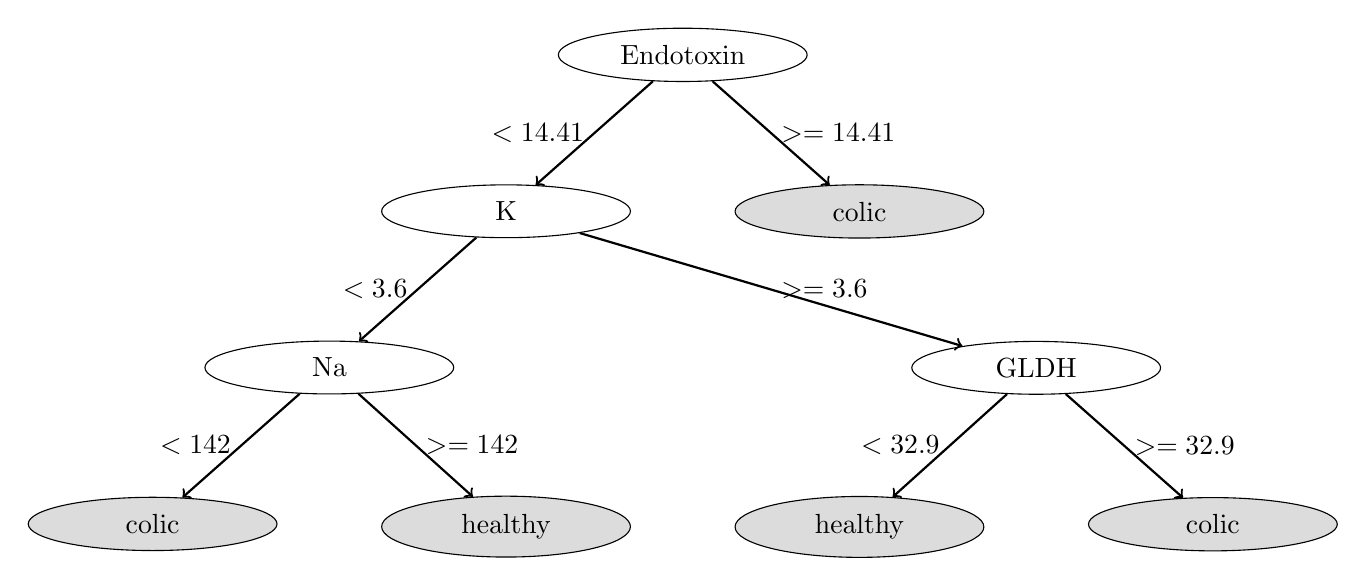
\begin{tikzpicture}[
  node distance=1.5cm and 0cm,
  mynode/.style={draw,ellipse,text width=2cm,align=center}]
\node[mynode] (en) {Endotoxin};
\node[mynode, below left=of en] (k) {K};
\node[mynode,  fill={rgb,255:red,220; green,220; blue,220}, below right=of en] (2c) {colic};
\node[mynode, below left=of k] (na) {Na};
\node[mynode, below right=of 2c] (gldh) {GLDH};
\node[mynode, fill={rgb,255:red,220; green,220; blue,220}, below left=of na] (4c) {colic};
\node[mynode, fill={rgb,255:red,220; green,220; blue,220}, below right=of na] (4h) {healthy};
\node[mynode, fill={rgb,255:red,220; green,220; blue,220}, below left=of gldh] (4hr) {healthy};
\node[mynode, fill={rgb,255:red,220; green,220; blue,220}, below right=of gldh] (4cr) {colic};


\path[->,draw,thick]
  (en) edge node[left=of en] {$< 14.41$} (k)
  (en) edge node[right=of en] {$>= 14.41$} (2c)
  (k) edge node[left=of en] {$< 3.6$} (na)
  (k) edge node[right=of en] {$>= 3.6$} (gldh)
  (na) edge node[left=of en] {$< 142$} (4c)
  (na) edge node[right=of en] {$>= 142$} (4h)
  (gldh) edge node[left=of en] {$< 32.9$} (4hr)
  (gldh) edge node[right=of en] {$>= 32.9$} (4cr);
 
\end{tikzpicture}
\newpage
\textbf{Q4.3)} For the training set we get that we correctly classifiy:
\[ \text{132 out of 132 training data points} \]
\textbf{Q4.4)} For the test set we get that we correctly classify:
\[ \text{13 our of the 13 testing data points} \]
\end{titlepage}
\end{document}